\documentclass[fleqn, 8pt]{amsart}
\usepackage[a4paper, margin = 1cm]{geometry}
\usepackage{exsheets} %question and solution environments
\usepackage{amsmath, amssymb, amsthm} %standard AMS packages
\usepackage[utf8]{inputenc}
\usepackage{esint} %integral signs
\usepackage{marginnote} %marginnotes
\usepackage{gensymb} %miscellaneous symbols
\usepackage{commath} %differential symbols
\usepackage{xcolor} %colours
\usepackage{cancel} %cancelling terms
\usepackage[free-standing-units,space-before-unit]{siunitx} %formatting units
	\sisetup
	{
		per-mode=fraction,
		fraction-function=\frac
	}
\usepackage{tikz, pgfplots} %diagrams
	\usetikzlibrary{calc, hobby, patterns, intersections, angles, quotes, spy}
\usepackage{graphicx} %inserting graphics
\usepackage{epstopdf} %converting and inserting eps graphics
\usepackage{hyperref} %hyperlinks
\usepackage{datetime} %date and time
\usepackage{ulem} %underline for \emph{}
\usepackage{xfrac, lmodern} %inline fractions
%\usepackage{enumerate, enumitem} %numbered lists
\usepackage{enumerate}
%\usepackage{enumitem}
\usepackage{float} %inserting floats
\usepackage[american voltages]{circuitikz} %circuit diagrams
\usepackage{pdflscape} %pages in landscape orientation
\usepackage{setspace} %double spacing
\usepackage{microtype} %micro-typography
\usepackage{listings} %formatting code
	\lstset{language=Matlab}
	\lstdefinestyle{standardMatlab}
	{
		belowcaptionskip=1\baselineskip,
		breaklines=true,
		frame=L,
		xleftmargin=\parindent,
		language=C,
		showstringspaces=false,
		basicstyle=\footnotesize\ttfamily,
		keywordstyle=\bfseries\color{green!40!black},
		commentstyle=\itshape\color{purple!40!black},
		identifierstyle=\color{blue},
		stringstyle=\color{orange},
	}
\usepackage{algpseudocode} %algorithms
\usepackage{algorithm} %algorithms
\usepackage{chronology}
\usepackage{qtree}
\usepackage{varwidth}
\usepackage{asymptote}
\usepackage{chemfig}
\usepackage{booktabs}
\usepackage{multirow}
\usepackage{titlesec}
\usepackage{todonotes}
\usepackage{placeins}
\usepackage{ifdraft}
%	\ifoptiondraft
%	{%
%		\doublespacing
%		\usepackage{showframe}
%	}
%	{%
%	    % nothing to be done here
%	}
\usepackage[extreme, title = normal]{savetrees}
\usepackage{multicol}
\usepackage{titlesec}

\renewcommand{\marginfont}{\scriptsize \color{red}}

\newcommand\numberthis{\addtocounter{equation}{1}\tag{\theequation}} %adds numbers to specific equations in non-numbered list of equations

\theoremstyle{definition}
\newtheorem{example}{Example}
\newtheorem{definition}{Definition}

\theoremstyle{theorem}
\newtheorem{theorem}{Theorem}
\newtheorem{law}{Law}

\newcommand{\curl}{\mathrm{curl\,}}

\newcommand{\divergence}{\mathrm{div\,}}

\newcommand{\normeq}{\stackrel{\|\cdot\|}{=}}

\DeclareMathOperator{\proj}{proj}
\DeclareMathOperator{\setspan}{span}

\makeatletter
\@addtoreset{section}{part} %resets section numbers in new part
\makeatother

\newcommand\blfootnote[1]{%
	\begingroup
	\renewcommand\thefootnote{}\footnote{#1}%
	\addtocounter{footnote}{-1}%
	\endgroup
}

\renewcommand{\tilde}{\widetilde}

\SetupExSheets{solution/print = true} %prints all solutions by default

% Uncomment to hide proofs
%\NewEnviron{killcontents}{}
%\let\proof\killcontents
%\let\endproof\endkillcontents

%opening
\title{Harmonic Analysis}
\author{Aakash Jog}
\date{2015-16}

\begin{document}

\maketitle
\setlength{\mathindent}{0pt}

\blfootnote
{	
	\begin{figure}[H]
		
\includegraphics[height = 12pt]{cc.eps}
		\includegraphics[height = 12pt]{by.eps}
		\includegraphics[height = 12pt]{nc.eps}
		\includegraphics[height = 12pt]{sa.eps}
	\end{figure}
	This work is licensed under the Creative Commons Attribution-NonCommercial-ShareAlike 4.0 International License. To view a copy of this license, visit \url{http://creativecommons.org/licenses/by-nc-sa/4.0/}.
} %CC-BY-NC-SA license

\begin{multicols}{2}

\begin{spacing}{0.7}

\part{Fourier Series}

\section{Fourier Series}

\begin{definition}[Real Fourier series]
	Let $f : [-L,L] \in \mathbb{C}$ be a piecewise continuous function.
	\fbox{$f(x) \approx \frac{a_0}{2} + \sum\limits_{n = 1}^{\infty} \left( a_n \cos(n x) + b_n \sin(n x) \right)$}
	\fbox{$f(x)  \approx \sum\limits_{n = -\infty}^{\infty} c_n e^{i n x}$}
	\fbox{$a_0 = \frac{1}{L} \int\limits_{-L}^{L} f(x) \dif x$}
	\fbox{$a_n = \frac{1}{L} \int\limits_{-L}^{L} f(x) \cos(n x) \dif x$}
	\fbox{$b_n = \frac{1}{L} \int\limits_{-L}^{L} f(x) \sin(n x) \dif x$}
	\fbox{$c_n = \frac{1}{2 L} \int\limits_{-L}^{L} f(x) e^{-i n x} \dif x$}
\end{definition}

\begin{definition}[Piecewise continuous functions]
	$f : \mathbb{R} \to \mathbb{R}$ is said to be piecewise continuous if, for every finite interval $[a,b]$ there is a finite number of discontinuity points, and the one-sided limits at each of these points are also finite.
\end{definition}

\begin{definition}[Piecewise continuously differentiable functions]
	$f : \mathbb{R} \to \mathbb{R}$ is said to be piecewise continuously differentiable if it is piecewise continuous, and
	\fbox{$\lim\limits_{h \to 0^+} \frac{f(x + h) - f(x^+)}{h} < \infty$}
	\fbox{$\lim\limits_{h \to 0^-} \frac{f(x - h) - f(x^-)}{h} < \infty$}
\end{definition}

\begin{theorem}[Bessel's Inequality]
	Let $f(x)$ be a piecewise continuous function defined on $[-L,L]$.
	Then
	\fbox{$\frac{1}{2} {a_0}^2 + \sum\limits_{n = 1}^{\infty} {a_n}^2 + {b_n}^2  \le \frac{1}{L} \int\limits_{-L}^{L} {f(x)}^2 \dif x$}
	\label{Bessel's_Inequality}
\end{theorem}

\begin{theorem}[Riemann-Lebesgue's Lemma]
	If $f(x)$ is piecewise continuous on $[-L,L]$, then
	\fbox{$\lim\limits_{n \to \infty} a_n = \lim\limits_{n \to \infty} b_n = 0$}
	\label{Riemann-Lebesgue's_Lemma}
\end{theorem}

\begin{definition}[Dirichlet kernel]
	\begin{equation*}
		D_m(t)  = \frac{1}{2} \sum\limits_{n = -m}^{m} e^{-i n t}
                        = \frac{1}{2} + \sum\limits_{n = 1}^{m} \cos(n t)
                        = \frac{\sin\left( \left( n + \frac{1}{2} \right) t \right)}{2 \sin \frac{t}{2}}
	\end{equation*}
	is called the Dirichlet kernel of order $m$.
\end{definition}

\begin{theorem}[Second representation of Dirichlet's kernel]
	Let $m \in \mathbb{N}$.\\
	Then, for $t \neq 2 \pi k$, where $k \in \mathbb{Z}$,
	\begin{equation*}
		D_m(t) = \frac{1}{2} + \cos(t) + \cos(2 t) + \dots + \cos(m t) = \frac{\sin\left( \left( m + \frac{1}{2} \right) t \right)}{2 \sin\left( \frac{1}{2} t \right)}
	\end{equation*}
\end{theorem}

\begin{theorem}
	Let
	\fbox{$S_m(f,x) = \frac{1}{2} a_0 + \sum\limits_{n = 1}^{m} a_n \cos(n x) + b_n \sin(n x)$}
	Then,
	\fbox{$S_m(f,x) = \frac{1}{\pi} \int\limits_{-\pi}^{\pi} f(x + t) \left( \frac{1}{2} \sum\limits_{n = 1}^{m} \cos(n t) \right) \dif t$}
\end{theorem}

\begin{theorem}[Dirichlet Theorem]
	Let $f : [-\pi,\pi] \to \mathbb{R}$ be a piecewise continuously differentiable function.\\
	Then, $\forall x \in (-\pi,\pi)$,
	\fbox{$\frac{1}{2} a_0 + \sum\limits_{n = 1}^{\infty} a_n \cos(n x) + b_n \sin(n x) = \frac{f(x^-) + f(x^+)}{2}$}
	and for $x = \pi$ or $x = -\pi$,
	\fbox{$\frac{1}{2} a_0 + \sum\limits_{n = 1}^{\infty} a_n \cos(n x) + b_n \sin(n x) = \frac{f(\pi^-) + f(-\pi^+)}{2}$}
	\label{Dirichlet_Theorem}
\end{theorem}

\begin{theorem}
	If $f$ is a piecewise continuous and periodic function with period of $2 \pi$, then
	\fbox{$S_m(x) = \frac{1}{\pi} \int\limits_{-\pi}^{\pi} f(x + t) D_m(t) \dif t$}
\end{theorem}

\begin{theorem}[Cauchy-Schwartz Inequality for Generalized Fourier Series]
	Let $u,v \in V$, where $V$ is an inner product space over $\mathbb{F}$.
	Then,
	\begin{align*}
		\left| \langle u,v \rangle \right| &\le \|u\| \|v\|
	\end{align*}
	\label{thm:Cauchy-Schwartz_Inequality_for_Generalized_Fourier_Series}
\end{theorem}

\begin{theorem}[Best Approximation Theorem]
	Let $\{u_i\}_{i = 1}^{n}$ be an orthonormal system in an normed inner product space $V$.
	Let $v \in V$.
	Then, $\forall \{c_i\}_{i = 1}^{n} \subset \mathbb{F}$,
	\begin{enumerate}
		\item $\left\| v - \sum\limits_{k = 1}^{n} \langle v,u_k \rangle u_k \right\|^2 \le \left\| v - \sum\limits_{k = 1}^{n} c_k u_k \right\|^2$
		\item $\left\| v - \sum\limits_{k = 1}^{n} \langle v,u_k \rangle u_k \right\|^2 = \|v\|^2 -  \sum\limits_{k = 1}^{n} \left| \langle v,u_k \rangle \right|^2$
	\end{enumerate}
	\label{thm:Best_Approximation_Theorem}
\end{theorem}

\section{Fourier Series in a General Interval}

\begin{definition}
	Let $f$ be a piecewise continuous function defined on $[a,b]$.
	The Fourier series over $[a,b]$ is defined as
	\fbox{$f(x) \approx \frac{a_0}{2} + \sum\limits_{n = 1}^{\infty} \left( a_n \cos\left( \frac{2 \pi n x}{b - a} \right) + b_n \sin\left( \frac{2 \pi n x}{b - a} \right) \right) \\$}
	\fbox{$f(x) \approx \sum\limits_{-\infty}^{\infty} c_n e^{\frac{2 \pi i n x}{b - a}}$}
	where
	\fbox{$a_0 = \frac{1}{b - a} \int\limits_{a}^{b} f(x) \dif x$}
	\fbox{$a_n = \frac{2}{b - a} \int\limits_{a}^{b} f(x) \cos \frac{2 \pi n x}{b - a} \dif x$}
	\fbox{$b_n = \frac{2}{b - a} \int\limits_{a}^{b} f(x) \sin \frac{2 \pi n x}{b - a} \dif x$}
	\fbox{$c_n = \frac{1}{b - a} \int\limits_{a}^{b} f(x) e^{\frac{2 \pi i n x}{b - a}} \dif x$}
\end{definition}

\begin{theorem}
	Let $f$ be continuous in $[-\pi,\pi]$, with piecewise continuous derivative, and $f(-\pi) = f(\pi)$.
	Then, the Fourier series converges uniformly on $[-\pi,\pi]$.
\end{theorem}

\begin{theorem}[Perceval Equality]
	Let $f$ be a piecewise continuous function in $[-\pi,\pi]$.
	Then,
	\fbox{$\frac{1}{\pi} \int\limits_{-\pi}^{\pi} \left| f(x) \right|^2 \dif x = \frac{{a_0}^2}{2} + \sum\limits_{n = 1}^{\infty} \left( {a_n}^2 + {b_n}^2 \right)$}
	\fbox{$\frac{1}{\pi} \int\limits_{-\pi}^{\pi} \left| f(x) \right|^2 \dif x = 2 \sum\limits_{n = -\infty}^{\infty} \left| c_n \right|^2$}
	\label{Perceval_Equality}
\end{theorem}

\begin{theorem}
	If $f$ is piecewise continuous with Fourier series
	\fbox{$f(x) \approx \frac{a_0}{2} + \sum\limits_{n = 1}^{\infty} a_n \cos(n x) + b_n \sin(n x)$}
	the, for all $x \in [-\pi,\pi]$,
	\fbox{$\int\limits_{0}^{x} f(t) \dif t = \frac{a_0}{2} x + \sum\limits_{n = 1}^{\infty} \frac{a_n}{n} \sin(n x) - \frac{b_n}{n} \left( \cos(n x) - 1 \right)$}
	This is not a Fourier series due to the $x$ in $\frac{a_0}{2} x$.\\
	Therefore, substituting the Fourier series of $x$,
	\begin{equation*}
		\int\limits_{0}^{x} f(t) \dif t = \sum\limits_{n = 1}^{\infty} \frac{b_n}{n} + \sum\limits_{n = 1}^{\infty} \left( \frac{a_n + (-1)^n a_0}{n} \sin(n x) - \frac{b_n}{n} \cos(n x) \right)
	\end{equation*}
\end{theorem}

\begin{theorem}[Bessel's Inequality for a General Interval]
	Let $f : [a,b] \to \mathbb{R}$ be a piecewise continuous function.
	Then,
	\begin{align*}
		\frac{1}{2} (a_0)^2 + \sum\limits_{n = 1}^{\infty} (a_n)^2 + (b_n)^2 &\le \frac{2}{b - a} \int\limits_{a}^{b} \left| f(x) \right|^2 \dif x\\
		\sum\limits_{n = -\infty}^{\infty} |c_n|^2 &\le \frac{1}{b - a} \int\limits_{a}^{b} \left| f(x) \right|^2 \dif x
	\end{align*}
	\label{thm:Bessel's_Inequality_for_a_General_Interval}
\end{theorem}

\begin{theorem}[Dirichlet's Theorem for a General Interval]
	Let $f : [a,b] \to \mathbb{R}$ be a piecewise continuously differentiable function.
	Then,
	\begin{align*}
		\frac{1}{2} a_0 + \sum\limits_{n = 1}^{\infty} a_n \cos\left( \frac{2 \pi}{b - a} n x \right) + b_n \sin\left( \frac{2 \pi}{b - a} n x \right)\\
		&= \sum\limits_{n = -\infty}^{\infty} c_n e^{i \frac{2 \pi}{b - a} n x}\\
		&= \frac{f\left( x^+ \right) + f\left( x^- \right)}{2}
	\end{align*}
	\label{thm:Dirichlet's_Theorem_for_a_General_Interval}
\end{theorem}

\begin{theorem}[Term-by-term Differentiation for a General Interval]
	Let $f : [a,b] \to \mathbb{R}$ be a piecewise continuous function, such that $f(a) = f(b)$, and $f'(x)$ is piecewise continuous.
	Then, if
	\begin{align*}
		f(x) &= \sum\limits_{n = -\infty}^{\infty} c_n e^{i \frac{2 \pi}{b - a} n x}
	\end{align*}
	then
	\begin{align*}
		f(x) &\approx \sum\limits_{n = -\infty}^{\infty} i \frac{2 \pi}{b - a} n c_n e^{i \frac{2 \pi}{b - a} n x}
	\end{align*}
	\label{thm:Term-by-term_Differentiation_for_a_General_Interval}
\end{theorem}

\begin{theorem}
	If $f$ is $2 \pi$ periodic and $k$ times differentiable, such that the $k$ derivatives are continuous and $f^{(k + 1)}(x)$ is piecewise continuous, then,
	\fbox{$\lim\limits_{n \to \infty} \left| n^k a_n \right| = \lim\limits_{n \to \infty} \left| n^k b_n \right| = \lim\limits_{n \to \infty} \left| n^k c_n \right| = 0$}
\end{theorem}

\begin{theorem}
	If the Fourier coefficients of a $2 \pi$ periodic function satisfy
	\fbox{$|c_n| \le \frac{c}{n^{k + 1 + \varepsilon}}$}
	where $\varepsilon > 0$, and $c$ is constant, then $f$ is $k$ times differentiable.
\end{theorem}

\begin{theorem}
	Let $k$ be the largest integer such that
	\fbox{$\lim\limits_{n \to \infty} n^k f(x) = 0$}
	Then, $f(x)$ is continuously differentiable at most $k$ times.
	Also, if
	\fbox{$f(x) \le \frac{1}{n^{k + 1 + \varepsilon}}$}
	then, $k$ is differentiable $k$ times.
\end{theorem}

\begin{theorem}[Term-by-term differentiation]
	Let the Fourier coefficients of $f(x)$ be $a_0$, $a_n$, $b_n$, $c_n$.
	Then, the Fourier coefficients of $f'(x)$ are
	\begin{align*}
		\alpha_0 &= 0\\
		\alpha_n &= n b_n\\
		\beta_n &= -n a_n\\
		\gamma_n &= i n c_n
	\end{align*}
\end{theorem}

\begin{theorem}[Term-by-term integration]
	Let
	\begin{align*}
		f(x) &= \frac{a_0}{2} + \sum\limits_{n = 1}^{\infty} a_n \cos(n x) + b_n \sin(n x)
	\end{align*}
	Then, the integral of $f(x)$ is
	\begin{align*}
		F(x) &\approx \frac{a_0}{2} x + \sum\limits_{n = 1}^{\infty} \frac{a_n \sin(n x) + b_n\left( 1 - \cos(n x) \right)}{n}
	\end{align*}
\end{theorem}

\section{Inner Product Spaces}

\begin{theorem}[Cauchy-Schwartz Inequality]
	\begin{align*}
		\left| \left\langle \overrightarrow{x},\overrightarrow{y} \right\rangle \right| &\le \left\| \overrightarrow{x} \right\| \left\| \overrightarrow{y} \right\|
	\end{align*}
	\label{thm:Cauchy-Schwartz_Inequality}
\end{theorem}

\begin{definition}[Norm]
	Let $V$ be a vector space.
	A function $\|\cdot\| : V \to \mathbb{R}^+$, such that
	\begin{enumerate}
		\item
			$\forall v \in V$,
			\fbox{$\|v\| \ge 0$}
			and $\|v\| = 0$ if an only if $v = \overrightarrow{0}$.
		\item
			$\forall v \in V$ and $\alpha \in \mathbb{F}$,
			\fbox{$\|\alpha v\| = |\alpha| \|v\|$}
		\item
			$\forall u,v \in V$,
			\fbox{$\|u + v\| \le \|u\| + \|v\|$}
	\end{enumerate}
	is called a norm.\\
	It is usually defined as
	\fbox{$\|v\| = \sqrt{\langle v,v \rangle}$}
\end{definition}

\begin{theorem}[Pythagoras Theorem]
	If $u,v \in V$ are orthogonal vectors in an inner product space, then
	\fbox{$\|u + v\|^2 = \|u\|^2 + \|v\|^2$}
	\label{thm:Pythagoras_Theorem}
\end{theorem}

\begin{definition}
	A set is said to be orthonormal if $\forall u,v \in V$,
	\fbox{$\langle u,v \rangle = 0$}
	and
	\fbox{$\|v\| = 1$}
\end{definition}

\begin{theorem}
	In the space $C^0[-\pi,\pi]$ with
	\fbox{$\langle f,g \rangle = \frac{1}{\pi} \int\limits_{-\pi}^{\pi} f(x) g(x) \dif x$}
	the set $\left\{ \frac{1}{\sqrt{2}} \right\} \cup \left\{ \cos(n x) \right\}_{n = 1}^{\infty} \cup \left\{ \sin(n x) \right\}_{n = 1}^{\infty}$ is orthonormal.
\end{theorem}


\begin{definition}[Orthonormal set]
	A set $\{c_1,\dots,c_n\}$ is said to be orthonormal if
	\fbox{$\langle c_i,c_j \rangle = \delta_{i j}$}
\end{definition}

\begin{definition}[Projection]
	Let $W$ be a subspace of a vector space $V$, such that
	\fbox{$W = \setspan\{c_1,\dots,c_n\}$}
	The projection of a vector $v$ with respect to $W$ is defined as
	\fbox{$\proj_{W}(v) = v_W = \sum\limits_{k = 1}^{n} \frac{\langle v,c_k \rangle}{\|c_k\|^2} c_k$}
\end{definition}

\begin{theorem}
	Let $W$ be a subspace of a vector space $V$.
	Let $v \in V$.\\
	Then, $v_W$ is the best approximation for $v$ in $W$, i.e.
	\fbox{$\left\| v - \proj_W(v) \right\| = \min\limits_{w \in W} \|v - w\|$}
\end{theorem}

\begin{theorem}
	Let $W$ be a subspace of a vector space $V$.
	Let $v \in V$.\\
	Then, $v - v_W \in W^{\perp}$, and $v_W \in W$.
\end{theorem}

\begin{theorem}
	Let $W$ be a subspace of a vector space $V$.
	Let $v \in V$.\\
	\fbox{$\|v\|^2 = \|v_W\|^2 + \left\| v - v_W \right\|^2$}
\end{theorem}

\begin{definition}[Complete set]
	An orthonormal set $\{u_k\}_{k = 1}^{\infty}$ is said to be complete if the only vector $v \in V$, such that $\forall k$,
	\fbox{$\langle v,u_k \rangle = 0$}
	is the zero vector.
\end{definition}

\begin{definition}[Closed system]
	Let $\{e_n\}_{n = 1}^{\infty}$ be an orthonormal system in $V$.
	The system is said to be a closed system if for each $u \in V$,
	\begin{align*}
		\lim\limits_{N \to \infty} \left\| u - \sum\limits_{n = 1}^{N} \langle u,e_n \rangle e_n \right\| &= 0
	\end{align*}
	Alternatively,
	\begin{align*}
		u &\normeq \sum\limits_{n = 1}^{\infty} \langle u,e_n \rangle e_n
	\end{align*}
\end{definition}

\begin{definition}[Continuity of functions]
	Let $f : V \to \mathbb{F}$.
	$f$ is said to be continuous at $v_0$ if for each $\varepsilon > 0$, $\exists \delta > 0$ such that $\forall v$ such that $\|v - v_0\| < \delta$, $\left| f(v) - f(v_0) \right| < \varepsilon$.
\end{definition}

\begin{theorem}
	The function $\langle \cdot,\cdot \rangle : V \times V \to \mathbb{F}$ is continuous with respect to both variables.
\end{theorem}

\begin{theorem}
	A closed orthonormal set is complete.
\end{theorem}

\begin{theorem}
	The sequence $\{S_k\}_{k = 1}^{\infty}$ where
	\begin{align*}
		S_k &= \sum\limits_{n = 1}^{k} \langle f,\varphi_n \rangle \varphi_n
	\end{align*}
	is a Cauchy sequence.
\end{theorem}

\begin{theorem}
	For a Hilbert space, a sequence is Cauchy if and only if it is converging.
\end{theorem}

\begin{definition}[Hilbert space]
	A inner product, normed, complete vector space is said to be a Hilbert space.
\end{definition}

\begin{theorem}[Central Theorem about Complete Orthonormal Systems]
	Let $V$ be a Hilbert space.
	Then, the following conditions are equivalent for an orthonormal set $\{u_k\}_{k = 1}^{\infty}$,
	\begin{enumerate}
		\item
			For $v \in V$, if $\forall k$,
			\fbox{$\langle v,u_k \rangle = 0$}
			then
			\fbox{$v = \overrightarrow{0}$}
			That is, if any vector is orthogonal to the entire orthonormal set, then the vector must be the zero vector.
		\item
			For $v \in V$,
			\fbox{$\lim\limits_{n \to \infty} \left\| \sum\limits_{k = 1}^{n} \langle v,u_k \rangle u_k - v \right\| = 0$}
		\item
			For $v \in V$,
			\fbox{$\sum\limits_{k = 1}^{\infty} \left| \langle v,u_k \rangle \right|^2 = \|v\|^2$}
			That is, Perceval's Equality holds.
	\end{enumerate}
\end{theorem}

\begin{question}
	Let
	\begin{align*}
		\lambda_n & = \min\limits_{\alpha \in \mathbb{R}} \frac{1}{\pi} \int\limits_{-\pi}^{\pi} \left| \sqrt{\cos x} - \alpha \cos(n x) \right|^2 \dif x
	\end{align*}
	Calculate $\lim\limits_{n \to \infty} \lambda_n$.
\end{question}

\begin{solution}
	\begin{align*}
		\langle f,g \rangle & = \frac{1}{\pi} \int\limits_{-\pi}^{\pi} f \overline{g} \dif x
	\end{align*}
	Therefore,
	\begin{align*}
		\langle f,f \rangle & = \frac{1}{\pi} \int\limits_{-\pi}^{\pi} f \overline{f} \dif x \\
                                    & = \frac{1}{\pi} \int\limits_{-\pi}^{\pi} |f|^2 \dif x
	\end{align*}
	Therefore, if
	\begin{align*}
		f(x) & = \sqrt{\cos x}
	\end{align*}
	then,
	\begin{align*}
		\lambda_n & = \min\limits_{\alpha \in \mathbb{R}} \left| \sqrt{\cos x} - \alpha \cos(n x) \right|^2 \\
                          & = \min\limits_{\alpha \in \mathbb{R}} \left| f(x) - \alpha \cos(n x) \right|^2
	\end{align*}
	Therefore, by the best approximation theorem, $\alpha$ will be the coefficient corresponding to the best approximation, i.e.,
	\begin{align*}
		\alpha \cos(n x) & = \proj_{W}\left( \sqrt{\cos x} \right)
	\end{align*}
	Therefore,
	\begin{align*}
		\alpha & = \frac{\left\langle \sqrt{\cos x},\cos(n x) \right\rangle}{\left\| \cos(n x) \right\|^2}
	\end{align*}
	Therefore,
	\begin{align*}
		\lambda_n & = \left\| \sqrt{\cos x} - \alpha \cos(n x) \right\|^2                                                                                                       \\
                          & = \left\| \sqrt{\cos x} - \frac{\left\langle \sqrt{\cos x},\cos(n x) \right\rangle}{\left\| \cos(n x) \right\|^2} \cos(n x) \right\|^2                      \\
                          & = \left\| \sqrt{\cos x} \right\|^2 - \frac{\left\langle \sqrt{\cos x},\cos(n x) \right\rangle^2}{\left\| \cos(n x) \right\|^2} \left\| \cos(n x) \right\|^2 \\
                          & = \left\| \sqrt{\cos x} \right\|^2 - \left\langle \sqrt{\cos x},\cos(n x) \right\rangle
	\end{align*}
	Therefore,
	\begin{align*}
		\left\| \sqrt{\cos x} \right\|^2 & = \frac{1}{\pi} \int\limits_{-\pi}^{\pi} |\cos x| \dif x                   \\
                                                 & = \frac{2}{\pi} \int\limits_{-\frac{\pi}{2}}^{\frac{\pi}{2}} \cos x \dif x \\
                                                 & = \frac{2}{\pi} \left. \sin x \right|_{-\frac{\pi}{2}}^{\frac{\pi}{2}}     \\
                                                 & = \frac{4}{\pi}
	\end{align*}
	Therefore,
	\begin{align*}
		\lambda_n & = \frac{4}{\pi} - {a_n}^2
	\end{align*}
	Therefore,
	\begin{align*}
		\lim\limits_{n \to \infty} \lambda_n & = \lim\limits_{n \to \infty} \left( \frac{4}{\pi} - {a_n}^2 \right) \\
                                                     & = \frac{4}{\pi} - \lim\limits_{n \to \infty} {a_n}^2
	\end{align*}
	By \nameref{Riemann-Lebesgue's_Lemma},
	\begin{align*}
		\lim\limits_{n \to \infty} a_n & = 0
	\end{align*}
	Therefore,
	\begin{align*}
		\lim\limits_{n \to \infty} \lambda_n & = \frac{4}{\pi}
	\end{align*}
\end{solution}

\begin{theorem}[Bessel's Inequality]
	Let $\{u_k\}_{k = 1}^{\infty}$ be an orthonormal system in $V$.
	Then, $\forall v \in V$,
	\begin{align*}
		\sum\limits_{k = 1}^{\infty} \left| \langle v,u_k \rangle \right|^2 &\le \|v\|^2
	\end{align*}
	\label{thm:Bessel's_Inequality}
\end{theorem}

\begin{theorem}[Perceval's Equality]
	The system $\{u_k\}_{k = 1}^{\infty}$ is a closed orthonormal system if and only if
	\begin{align*}
		\sum\limits_{k = 1}^{\infty} \left| \langle v,u_k \rangle \right|^2 &= \|v\|^2
	\end{align*}
	\label{thm:Perceval's_Equality}
\end{theorem}

\part{Integral Identities}

\begin{align*}
	\int u \sin u \dif u &= \sin u - u \cos u + c\\
	\int u \cos u \dif u &= \cos u + u \sin u + c\\
	\int u^2 \sin u \dif u &= 2 u \sin u + \left( 2 - u^2 \right) \cos u + c\\
	\int u^2 \cos u \dif u &= 2 u \cos u + \left( u^2 - 2 \right) \sin u + c\\
	\int e^{a x} \sin(p x) \dif x &= \frac{e^{a x} \left( a \sin(p x) - p \cos(p x) \right)}{a^2 + p^2}\\
	\int e^{a x} \cos(p x) \dif x &= \frac{e^{a x} \left( a \cos(p x) + p \sin(p x) \right)}{a^2 + p^2}\\
	\int \cos(m u) \cos(n u) \dif u &= \frac{\sin\left( (m + n) u \right)}{2 (m + n)} + \frac{\sin\left( (m - n) u \right)}{2 (m - n)} + c\\
	\int \sin(m u) \cos(n u) \dif u &= -\frac{\cos\left( (m + n) u \right)}{2 (m + n)} - \frac{\cos\left( (m - n) u \right)}{2 (m - n)} + c\\
	\int \sin(m u) \sin(n u) \dif u &= -\frac{\sin\left( (m + n) u \right)}{2 (m + n)} + \frac{\sin\left( (m - n) u \right)}{2 (m - n)} + c\\
	\int u e^{a u} \dif u &= \frac{e^{a u}}{a^2} (a u - 1) + c\\
	\int u^m e^{a u} \dif u &= \frac{u^m e^{a u}}{a} - \frac{m}{a} \int u^{m - 1} e^{a u} \dif u + c
\end{align*}

\begin{align*}
	\int x^a \dif x &= \frac{x^{a + 1}}{a + 1} + c\\
	\int \frac{\dif x}{x} &= \ln|x| + c\\
	\int e^x \dif x &= e^x + c\\
	\int a^x \dif x &= \frac{a^x}{\ln a} + c
\end{align*}

\begin{align*}
	\int \sin x \dif x &= -\cos x + c\\
	\int \cos x \dif x &= \sin x + c\\
	\int \sec x \dif x &= \tan x + c\\
	\int \csc x \dif x &= -\cot x + c\\
	\int \tan x \dif x &= -\ln|\cos x| + c\\
	\int \cot x \dif x &= \ln|\sin x| + c
\end{align*}

\begin{align*}
	\int \frac{1}{1 + x^2} \dif x &= \tan^{-1} x + c\\
	\int \frac{1}{\sqrt{1 - x^2}} \dif x &= \sin^{-1} x + c
\end{align*}

\begin{align*}
	\int \csc x \dif x &= \ln\left| \tan \frac{x}{2} \right| + c\\
	\int \sec x \dif x &= \ln\left| \tan\left( \frac{x}{2} + \frac{\pi}{4} \right) \right| + c
\end{align*}

\begin{align*}
	\int \frac{1}{a^2 + x^2} \dif x &= \frac{1}{a} \tan^{-1} \frac{x}{a} + c\\
	\int \frac{1}{x^2 - a^2} \dif x &= \frac{1}{2 a} \ln\left| \frac{x - a}{x + a} \right| + c\\
	\int \frac{1}{a^2 - x^2} \dif x &= \frac{1}{2 a} \ln\left| \frac{x + a}{x - a} \right| + c\\
	\int \frac{1}{\sqrt{x^2 \pm a^2}} \dif x &= \ln\left| x + \sqrt{x^2 + a^2} \right| + c\\
	\int \sqrt{a^2 - x^2} \dif x &= \frac{x}{2} \sqrt{a^2 - x^2} + \frac{a^2}{2} \sin^{-1} \frac{x}{a} + c\\
	\int \sqrt{x^2 \pm a^2} \dif x &= \frac{x}{2} \sqrt{x^2 + a^2} + \frac{a^2}{2} \ln\left| x + \sqrt{x^2 \pm a^2} \right| + c
\end{align*}

\begin{align*}
	\int\limits_{-L}^{L} \cos\left( \frac{m \pi}{L} x \right) \cos\left( \frac{n \pi}{L} x \right) \dif x &=
		\begin{cases}
			0 &;\quad m \neq n\\
			L &;\quad m = n \neq 0\\
			2 L &;\quad m = n = 0\\
		\end{cases}\\
	\int\limits_{-L}^{L} \sin\left( \frac{m \pi}{L} x \right) \cos\left( \frac{n \pi}{L} x \right) \dif x &= 0\\
	\int\limits_{-L}^{L} \sin\left( \frac{m \pi}{L} x \right) \sin\left( \frac{n \pi}{L} x \right) &=
		\begin{cases}
			0 &;\quad m \neq n\\
			L &;\quad m = n\\
		\end{cases}
\end{align*}

\part{Trigonometric Identities}

\begin{align*}
	\cos(2 a) &= 1 - 2 \sin^2 a\\
	&= 2 \cos^2 a - 1\\
	\sin(a \pm b) &= \sin a \cos b \pm \cos a \sin b\\
	\cos(a \pm b) &= \cos a \cos b \mp \sin a \sin b\\
	\sin^2 a + \cos^2 a &= 1\\
	\sec^2 a &= 1 + \tan^2 a\\
	\csc^2 a &= 1 + \cot^2 a\\
	\sin a \sin b &= \frac{\cos(a - b) - \cos(a + b)}{2}\\
	\sin a \cos b &= \frac{\sin(a + b) + \sin(a - b)}{2}\\
	\cos a \cos b &= \frac{\cos(a + b) + \cos(a - b)}{2}
\end{align*}

\end{spacing}

\end{multicols}

\end{document}
